\documentclass[a4paper]{article}

\usepackage{amsmath}
\usepackage{amsfonts}
\usepackage{graphicx}
\usepackage{color}

\newcommand{\blue}[1]{{\color{blue}#1}}
\newcommand{\R}{{\mathbb R}}

\addtolength{\textwidth}{4cm}
\addtolength{\textheight}{4cm}
\hoffset-2cm
\voffset-2cm

\begin{document}
\section{Preliminaries}
The authors use a nice consequent notation. Aside from the usual
derivatives and partial derivatives, for discontinuous variables, they
adopt the convention that $x^-$ is the value before the jump and $x^+$
the value after. One can formally define this as $x^- = \lim_{n \to
  \infty} x(t^* - \frac{1}{n})$ and $x^+ = \lim_{n \to
  \infty} x(t^* + \frac{1}{n})$, if the jump is at $t^*$.

Throughout the derivation, things remain contained within these
sensible notations without reference to non-existing derivatives at
the jump.

Throughout this manuscript, vectors do not have a separate
notation, so it is up to the reader to remember, which symbols are
vector-valued. The $\cdot$ is the normal scalar product on ${\mathbb
  R}^n$, i.e. $y\cdot z = \sum_{i=1}^n y_iz_i$.

I am not 100\% convinced that the use of normal and partial derivative
symbols is always following the most consequent line - we will discuss
when we see issues.

The original text is in \blue{blue} but I have at times corrected a
typo or added a detail (very minor changes). The black text is
commentary from me about what I think is going on.



\subsection{Overall approach}
There is a couple of main ideas that make the body of the method.
\begin{enumerate}
\item The adjoint method itself. For this Wunderlich and Pehle refer
  to \\
  63. Pontryagin, L.~S.~Mathematical Theory of Optimal Processes (Routledge,1962).\\
  64. Bradley, A.~M.~PDE-constrained optimization and the adjoint method (2019).\\
  I.e. we are looking at gradient descent in constrained optimisation
  problems. We will see Lagrange multipliers here but I think it is
  probably a distraction to try to find an intuition what the Lagrange
  multipliers $\lambda$ ``mean''. In this work, the goal is to regroup
  the calculations for the gradient of the loss function, which
  involves a huge number of forward derivatives $\frac{\partial
    x}{\partial p_i}$ (in the general formulation of a dynamical system
  $x(t)$) into a less computationally expensive backward pass of ``adjoint
  variables''. The trick is to indtroduce the Lagrange multipliers and
  then reformat everything so that they replace the need for
  tracking those many derivatives.
\item To do the adjoint method for a network of LIF neurons, one
  needs to work around the discontinuities of the spikes and look at
  how terms in the loss that depend on the spike time can be
  handled. The former is done by careful consideration of the jumps at
  spike times (and breaking everything up into differentiable periods
  and jump times). The latter involves using the implicit function
  theorem.
\item Finally, the previous point often takes the form of taking a jump
  condition, using that the jump occurs at $t^{\text{post}}_k$, which
  by the implicit function theorem is a differentiable function of the
  weights, and deriving relationships for $\frac{\partial
    \cdot}{\partial w_{ji}}$ that have the form of a direct partial
  derivative with respect to $w_{ji}$ plus a term that comes about
  through the dependence on $t^{\text{post}}_k$ (see for instance
  \blue{(36)}).
\end{enumerate}

\section{Adjoint method}

\blue{ We apply the adjoint method to a continuous, first order system of ordinary differential
equations and refer the reader to [63,64] for a more general setting. Consider an N-dimensional dynamical system
$x : t  \rightarrow x(t) \in \R^N$ with parameters $p \in \R^P$
defined by the system of implicit first order ordinary differential 
equations
\begin{align}
\dot{x} - F(x,p) = 0 \tag{15} \label{eq:dyn}
\end{align}
and constant initial conditions $G(x(0)) = 0$ where $F$, $G$ are smooth vector-valued functions.
}

For what follows it might be useful to think of this alternatively in
terms of the implicit function theorem where the $N$-dimensional
dynamical system might be defined as
\begin{align}
  {\cal F}(\dot{x}, x, p) = 0  \label{eq:dyn2}
\end{align}
with ${\cal F}(\dot{x}, x, p) = \dot{x} - F(x,p)$. More about this
when we discuss adding $\lambda \cdot {\cal F}$ to the loss function
$\cal L$.

\blue{We are interested in computing the gradient of a loss that is
  the integral of a smooth function l over the trajectory of x,
  \begin{align}
    {\cal L} =\int_0^T l(x,t) dt \tag{16}
  \end{align}
  We have
  \begin{align}
    \frac{d{\cal L}}{dp_i} = \int_0^T \frac{\partial l}{\partial x}
    \cdot \frac{\partial x}{\partial p_i} dt, \tag{17}
  \end{align}
  where $\cdot$ is the dot product ...
}

To unpack this, first, differentiation with respect to $p_i$ can be
swapped with the integration:
\begin{align}
  \frac{d}{dp_i} \int_0^T l(x,t) dt = \int_0^T \frac{d}{dp_i} l(x,t) dt
\end{align}
because the only dependency on $p_i$ is through $x$, which depends on
$p_i$ through the dynamics \blue{(\ref{eq:dyn})}. In other words the
integration limits $0$ and $T$ do not depend on $p_i$.

Then, it is chain rule,
\begin{align}
  \frac{d}{dp_i} l(x,t) = \sum_k \frac{\partial l}{\partial x_k}
   \frac{\partial x_k}{\partial p_i}
\end{align}
which can then be written using the scalar product in vector form,
\begin{align}
  \frac{\partial l}{\partial x}
  \cdot \frac{\partial x}{\partial p_i}
\end{align}
\blue{... and the dynamics of the partial derivatives $\frac{\partial
    x}{\partial p_i}$ are given by applying Gronwall’s theorem [61],
  \begin{align}
    \frac{d}{dt} \frac{\partial x}{\partial p_i} = \frac{\partial
      F}{\partial x}\frac{\partial x}{\partial p_i} + \frac{\partial
      F}{\partial p_i} . \tag{18}
  \end{align}
}

I believe Gronwall's theorem boils down to that under sufficient
smoothness assumptions, one can swap derivatives if taking the partial
derivatives of the dynamics equations \blue{(\ref{eq:dyn})},
\begin{align}
 & \dot{x} = F(x,p) \\
\Rightarrow \; &\frac{\partial }{\partial p_i} \frac{d x}{dt} =
\frac{\partial }{\partial p_i} F(x,p) \\
\Rightarrow \; &\frac{d}{dt} \frac{\partial x}{\partial p_i} = \frac{\partial }{\partial p_i} F(x,p) 
\end{align}
and then it is chain rule,
\begin{align}
\frac{\partial }{\partial p_i} F(x,p) = \frac{\partial
      F}{\partial x} \cdot \frac{\partial x}{\partial p_i} + \frac{\partial
  F}{\partial p_i}
\end{align}
where $\cdot$ is the scalar product (missing in the original text).

\blue{Computing $x(t)$ along with $\frac{\partial x}{\partial p_i}
  (t)$ using Eqs. (15) and (18) allows us to calculate the gradient in
  Eq. (17) in a single forward pass. However, this procedure can incur
  prohibitive computational cost. When considering a recurrent 
 neural network with $N$ neurons and $P = N^2$ synaptic weights,
 computing  $\frac{\partial x}{\partial p_i} (t)$ for all parameters
 requires storing and integrating $PN = N^3$ partial derivatives.
}

Note that \blue{(18)} is not needed for the adjoint method below and is only
there to make the point that one can in principle do feed-forward
gradient calculations. 

\blue{
 The adjoint method allows us to avoid computing PN partial
 derivatives in the forward pass by instead computing
 $N$ adjoint variables $\lambda (t)$ in an additional backward
 pass. We add a Lagrange multiplier $\lambda: t  \rightarrow
  \lambda(t) \in \R^N$ that constrains the system dynamics as given in Eq. (15),
 \begin{align}
   {\cal L} = \int_0^T \left[ l(x,t) + \lambda \cdot \left(\dot{x} -
     F(x,p)\right)\right] dt \tag{19}
 \end{align}
 Along trajectories where Eq.~(15) holds, $\lambda$ can be chosen arbitrarily
without changing $\cal L$ or its derivative.
}

This is a key step and I find it difficult to develop the right
intuition. I think the motivation for adding the langrange multiplier
is the eventual result of the reformulated derivative of the cost
function \blue{(24)}. I could not come up with a different motivation
or explanation why this is needed or what it is for.

To unpack the last statement a little, one can add the Langrange
multiplier without 
changing $\cal L$ because $\cal L$ is meant to only be calculated for
valid trajectories and for those ${\cal F}= \dot{x} - F(x,p) \equiv 0$ by
definition (see \blue{(\ref{eq:dyn})}).

For the derivative with respect to parameters
$\frac{\partial}{\partial p_i} \left(\dot{x} - F(x,p)\right)$ it may seem less
clear but if we think of the trajectories of the dynamical system for
two nearby values of $p_i$, then we know that for both ${\cal F}
\equiv 0$. So, therefore, there is no change of $\cal F$ with respect
to $p_i$, and hence the derivative of $\cal F$ with respect to $p_i$
is also $0$.

\blue{We
  get
  \begin{align}
    \frac{d \cal L}{d p_i} = \int_0^T \left[
      \frac{\partial l}{\partial x}\cdot \frac{\partial x}{\partial
        p_i} + \lambda \cdot \left(\frac{d}{dt}\frac{\partial
        x}{\partial p_i} - \frac{\partial F}{\partial x}\cdot
      \frac{\partial x}{\partial p_i} - \frac{\partial F}{\partial
        p_i}\right) \right] dt \tag{20}
  \end{align}
  }

Here, it is again the same argument as above for pulling the
derivative into the integral. Then, the term $\frac{\partial
  l}{\partial x}\cdot \frac{\partial x}{\partial p_i}$ is as in
\blue{(17)} and the term $\lambda \cdot \left(\frac{d}{dt}\frac{\partial
  x}{\partial p_i} - \frac{\partial F}{\partial x}\cdot
\frac{\partial x}{\partial p_i} - \frac{\partial F}{\partial
  p_i}\right)$ uses the same arguments as previously in
\blue{(18)} (see above).

\blue{Using partial integration, we have
  \begin{align}
    \int_0^T \lambda \cdot \frac{d}{dt} \frac{\partial x}{\partial
      p_i} dt = - \int_0^T \dot{\lambda} \cdot \frac{\partial x}
    {\partial p_i} dt +\left[\lambda \cdot \frac{\partial x}{\partial
        p_i} \right]^T_0 . \tag{21}
  \end{align}
  
}

Just to be sure, partial integration is
\begin{align}
  \int u(t) \dot{v}(t) dt = \left[ u(t) v(t) \right] - \int \dot{u}(t) v(t)
  dt
\end{align}
with $u(t) = \lambda (t)$, $v(t) = \frac{\partial x}{\partial p_i}$
this yields \blue{(21)}.

\blue{
  By setting  $\lambda(T) = 0$, the boundary term vanishes because we
  chose parameter independent initial conditions ($\frac{\partial
    x}{\partial p_i} = 0$). The gradient becomes
  \begin{align}
    \frac{d \cal L}{d p_i} = \int_0^T \left[\left( \frac{\partial
        l}{\partial x} - \dot{\lambda} - \frac{\partial F}{\partial x}
      \lambda \right) \cdot \frac{\partial x}{\partial p_i} - \lambda
      \cdot \frac{\partial F}{\partial p_i} \right] dt .
  \end{align}
}

I think this reveals the overall design of the method. When
starting out with \blue{(17)} we had to track the numerous and hence
inconvenient $\frac{\partial x}{\partial p_i}$. To get rid of that, we
use the Langrange multiplier and partial integration so that
$\frac{\partial x}{\partial p_i}$ is prefaced with a factor that we
can make identically $0$ along the whole trajectory with an
appropriate choice of $\lambda(t)$.

\blue{
  By choosing $\lambda$  to fulfill the adjoint differential equation
  \begin{align}
    \dot{\lambda} = \frac{\partial l}{\partial x} - \frac{\partial
      F}{\partial x} \lambda \tag{23} 
  \end{align}
  we are left with
  \begin{align}
    \frac{d \cal L}{d p_i} = - \int_0^T \lambda \cdot \frac{\partial
      F}{\partial p_i} dt . \tag{24}
  \end{align}
  The gradient can therefore be computed using Eq. (24), where the
  adjoint state variable $\lambda $  is computed from
$t = T$ to $t = 0$ as the solution of the adjoint differential equation Eq. (23) with initial condition  $\lambda(T) = 0$ . This
corresponds to backpropagation through time (BPTT) in discrete time artificial neural networks.
}

Mostly straightforward except the time inversion, maybe. My
understanding is that this is necessary only because we know the
``boundary condition'' at $T$ rather than at $0$: $\lambda (T) =
0$. This stems from the need to get rid of the boundary values during
the partial integration. To ensure this boundary condition, it is
easiest to make it the initial condition for a backwards integration
of the $\lambda$ dynamics \blue{(23)}.  

One way of summarising the method is to say $\lambda$ and its dynamics
backward in time cleverly combine what normally the many
$\frac{\partial x}{\partial p_i}$ would have contributed to the
gradient of the loss function.

\section{Gradient of the loss function of an SNN}

\blue{We apply the adjoint method (see previous methods subsection) to
  the case of a  spiking neural network (i.e., a hybrid, discontinuous
  system with parameter dependent state transitions). The  following
  derivation is specific to the model given in Table 1. A fully
  general treatment of (adjoint) sensitivity analysis in hybrid
  systems can be found in [8] or [10].

The differential equations defining the free dynamics in implicit form are
\begin{align}
  f_V \equiv \tau_{\text{mem}} \dot{V} + V - I = 0, \tag{25a} \\
  f_I \equiv \tau_{\text{syn}} \dot{I} + I = 0, \tag{25b}
\end{align}
where $f_V$, $f_I$ are again vectors of size $N$.
}

These are standard equations for $N$ leaky integrate and fire (LIF)
neurons and current-based synapses with exponential decay. The
corresponding transitions during a spike are described in the earlier
table 1, when $V_n - \vartheta = 0$ and $\dot{V}_n \neq 0$,
\begin{align}
  V^+_n &= 0 \label{eq:jumpV} \\
  I^+ &= I^- + W \cdot e_n \label{eq:jumpI}
\end{align}
where $e_n$ is the unit vector with a $1$ in dimension $n$ and $0$
otherwise. I.e., the voltage reset is to $0$ and post-synaptic input
currents are incremented by the sum of incoming weights from the
spiking neuron.

\blue{
  We now split up the loss integral in Eq. (1) at the spike times
  $t^{\text{post}}$ and use vectors of Lagrange multipliers
    $\lambda_V$, $\lambda_I$ that fix the system dynamics $f_V$, $f_I$
    between transitions. 
    \begin{align}
      \frac{d \cal L}{d w_{ji}} = \frac{d}{d w_{ji}} \left[
        l_p (t^{\text{post}}) + \sum_{k=0}^{N_{\text{post}}}
        \int_{t_k^{\text{post}}}^{t_{k+1}^{\text{post}}} [l_V(V,t) +
          \lambda_V \cdot f_V + \lambda_I \cdot f_I ] dt \right], \tag{26}
    \end{align}    
    where we set $t_0^{\text{post}} = 0$ and
    $t_{N_{\text{post}}+1}^{\text{post}} = T$ and $x \cdot y$ is the
    dot product of two vectors x, y. Note that because $f_V$, $f_I$ 
 vanish along all considered trajectories, $\lambda V$ and $\lambda I$
 can be chosen arbitrarily without changing $\cal L$ or its derivative. 
}

For reference, Eq. \blue{(1)} was:
\blue{
  \begin{align} 
    {\cal L} = l_p(t^{\text{post}}) + \int_0^T l_V(V(t),t) dt \tag{1}
  \end{align}
}
This is essentially the same approach as in the previous section
except that there are now two dynamics equations. The argument, why the
Lagrange multipliers can be added, are, however, exactly the
same. Another two notes would be (1) the $l_p$ term depends on all
post-synaptic spike times, i.e. $t^{\text{post}}$ without lower index
is the vector of all post-synaptic spike times, and (2) the splitting
of the integral for now does nothing but anticipates that later jumps
occur in some variables at the spike times and splitting the integral
into bits that are unproblematic inside helps dealing with these
discrete events.

\blue{
  Using Eq. (25) we have, as per Gronwall’s theorem [61],
  \begin{align}
    \frac{\partial f_V}{\partial w_{ji}} &= \tau_{\text{mem}}
    \frac{d}{dt} \frac{\partial V}{\partial w_{ji}} + \frac{\partial
      V}{\partial w_{ji}} - \frac{\partial I}{\partial
      w_{ji}}, \tag{27a}  \\ 
    \frac{\partial f_I}{\partial w_{ji}} &= \tau_{\text{syn}}
    \frac{d}{dt} \frac{\partial I}{\partial w_{ji}} +\frac{\partial
      I}{\partial w_{ji}}, \tag{27b}
  \end{align}
  where we have used the fact that the derivatives commute,
  $\frac{\partial }{\partial w_{ji}} \frac{d}{dt} = \frac{d}{dt}
  \frac{\partial }{\partial w_{ji}}$ (the weights are fixed and have
  no time dependence). 
}

I think the commuting of the derivatives is the essence of Gronwall's
theorem but it is commendable that they have considered that this only
works if $w_{ji}$ do not depend on $t$. Other than the swapping of
derivatives nothing special is happening here.

\blue{The gradient then becomes, by application of the Leibniz
  integral rule,
  \begin{align}
    \frac{d \cal L}{d w_{ji}} = &\sum_{k=0}^{N_{\text{post}}} \left[
      \int_{t_k^{\text{post}}}^{t_{k+1}^{\text{post}}} \left[
        \frac{\partial l_V}{\partial V} \cdot \frac{\partial
          V}{\partial w_{ji}} + \lambda_V \cdot \left(
        \tau_{\text{mem}} \frac{d}{dt} \frac{\partial V}{\partial
          w_{ji}} +\frac{\partial V}{\partial w_{ji}} - \frac{\partial
          I}{\partial w_{ji}}\right) + \lambda_I \cdot
        \left(\tau_{\text{syn}} \frac{d}{dt} \frac{\partial
          I}{\partial w_{ji}} + \frac{\partial I}{\partial w_{ji}}
        \right)\right] dt \right. \nonumber  \\
      & \left. + \frac{\partial l_p}{\partial t_k^{\text{post}}} \frac{d
        t_k^{\text{post}}}{d w_{ji}} + l^-_{V,k+1}
      \frac{dt_{k+1}^{\text{post}}}{d w_{ji}} - l^+_{V,k} \frac{d
        t_k^{\text{post}}}{d w_{ji}} \right], \tag{28}
  \end{align}
  
    where $l^{\pm}_{V,k}$ is the voltage-dependent loss evaluated before (-) or after ( + ) the transition and we have used that
    $f_V = f_I = 0$ along all considered trajectories.
    }

There is a lot to unpack here. The first thing to note is that the
integral boundaries $t_k^{\text{post}}$ and $t_{k+1}^{\text{post}}$
depend on $w_{ji}$ and hence the invocation of the Leibniz integral
rule. It is an interesting case where we have something of the type
\begin{align}
  \frac{d}{dx} \int_{f(x)}^{g(x)} h(x,t) dt &= \frac{d}{dx} \left(H(x,g(x)) - H(x,f(x))\right) \\
  &= \frac{\partial H}{\partial g} \frac{dg}{dx}\Big|_{x,g(x)} + \frac{\partial
    H}{\partial x}\Big|_{x,g(x)} - \frac{\partial H}{\partial f}
  \frac{df}{dx}\Big|_{x,f(x)} - \frac{\partial H}{\partial x}\Big|_{x,f(x)} \\
  &= h(x,g(x))\frac{dg(x)}{dx} - h(x,f(x)) \frac{df(x)}{dx} +
  \int_{f(x)}^{g(x)} \frac{\partial
    h}{\partial x} dt
\end{align}
So, the first row of \blue{(28)} is a straight-forward derivative of
the integrand with application of the chain rule, as well
as using \blue{(27a)} and \blue{(27b)}. That leaves the derivative of the
$l_p(t^{\text{post}})$ term and the terms caused by the
$w_{ji}$-dependent integration bounds. The former is a straightforward
application of the chain 
rule giving the term $\frac{\partial l_p}{\partial t_k^{\text{post}}}
\frac{d t_k^{\text{post}}}{d w_{ji}}$. For the latter we get
\begin{align}
 \big( l^-_{V,k+1}  +\lambda_V \cdot
  f_V(V^-_{k+1}) +\lambda_I \cdot f_I(I^-_{k+1})\big)\frac{dt_{k+1}^{\text{post}}}{d w_{ji}} - \big(l^+_{V,k}
   + f_V(V^+_{k}) + \lambda_I \cdot
  f_I(I^+_{k})\big) \frac{dt_k^{\text{post}}}{d w_{ji}}.  
\end{align}
However, all the terms with containing $f_V$ and $f_I$ are zero.

\blue{
  Using partial integration, we have
  \begin{align}
    \int_{t_k^{\text{post}}}^{t_{k+1}^{\text{post}}} \lambda_V \cdot
    \frac{d}{dt} \frac{\partial V}{\partial w_{ji}} dt =
    - \int_{t_k^{\text{post}}}^{t_{k+1}^{\text{post}}} \dot{\lambda}_V
\cdot \frac{\partial V}{\partial w_{ji}} dt + \left[\lambda_V \cdot
  \frac{\partial V}{\partial w_{ji}}
  \right]_{t_k^{\text{post}}}^{t_{k+1}^{\text{post}}} , \tag{29} \\
    \int_{t_k^{\text{post}}}^{t_{k+1}^{\text{post}}} \lambda_I \cdot
    \frac{d}{dt} \frac{\partial I}{\partial w_{ji}} dt =
    - \int_{t_k^{\text{post}}}^{t_{k+1}^{\text{post}}} \dot{\lambda}_I
\cdot \frac{\partial I}{\partial w_{ji}} dt + \left[\lambda_I \cdot
  \frac{\partial I}{\partial w_{ji}}
  \right]_{t_k^{\text{post}}}^{t_{k+1}^{\text{post}}}. \tag{30}
  \end{align}
  }

Very similar as in the more general derivation of the adjoint method
above except that here we cannot get rid of all the integrated terms
at $t_k^{\text{post}}$ and $t_{k+1}^{\text{post}}$ arguing that either
the $\lambda$'s or derivatives are $0$.

\blue{
  Collecting terms in $\frac{\partial V}{\partial w_{ji}}$,
  $\frac{\partial I}{\partial w_{ji}}$, we have
  \begin{align}
    \frac{d \cal L}{d w_{ji}} &= \sum_{k=0}^{N_{\text{post}}} \left[
      \int_{t_k^{\text{post}}}^{t_{k+1}^{\text{post}}} \left[\left(
        \frac{\partial l_V}{\partial V} - \tau_{\text{mem}}
        \dot{\lambda}_V + \lambda_V \right) \cdot \frac{\partial
          V}{\partial w_{ji}} + \left( - \tau_{\text{syn}}
        \dot{\lambda}_I + \lambda_I - \lambda_V \right) \cdot
        \frac{\partial I}{\partial w_{ji}} \right] dt
      \right. \nonumber \\
      & \left. + \frac{\partial l_p}{\partial t_k^{\text{post}}} \frac{d
        t_k^{\text{post}}}{d w_{ji}}
      +\tau_{\text{mem}} \left[ \lambda_V \cdot \frac{\partial
          V}{\partial w_{ji}}
        \right]_{t_k^{\text{post}}}^{t_{k+1}^{\text{post}}}
      +\tau_{\text{syn}} \left[\lambda_I \cdot \frac{\partial
          I}{\partial w_{ji}} \right]_{t_k^{\text{post}}}^{t_{k+1}^{\text{post}}}
      + l^-_{V,k+1}
      \frac{dt_{k+1}^{\text{post}}}{d w_{ji}} - l^+_{V,k} \frac{d
        t_k^{\text{post}}}{d w_{ji}} \right]. \tag{31}
  \end{align}
}
This is just straightforward term collections.

\blue{
  Since the Lagrange multipliers $\lambda_V(t)$, $\lambda_I(t)$ can be
  chosen arbitrarily, this form allows us to set the dynamics of 
the adjoint variables between transitions. Since the integration of the adjoint variables is done from $t = T$ to
$t = 0$ in practice (i.e., reverse in time), it is practical to
transform the time derivative as $\frac{d}{dt} \rightarrow
-\frac{d}{dt}$. Denoting the new time derivative by $'$, we have
\begin{align}
  \tau_{\text{mem}} \lambda'_V = -\lambda_V - \frac{\partial
    l_V}{\partial V}, \tag{32a} \\
  \tau_{\text{syn}} \lambda'_I = -\lambda_I + \lambda_V. \tag{32b}
\end{align}
The integrand in Eq. (31) therefore vanishes along the trajectory and
we are left with a sum over the transitions.
}

Exactly the same as previously but note how the signs have been
flipped to do the backward derivatives.

\blue{
  Since the initial conditions of V and I are assumed to be parameter
  independent, we have $\frac{\partial V}{\partial w_{ji}} =
  \frac{\partial I}{\partial w_{ji}} = 0$ at $t= 0$. We set the
  initial condition for the adjoint variables to be $\lambda_V(T) =
  \lambda_I(T) = 0$ to eliminate the boundary term for $t = T$ . We
  are, therefore, left with a sum over transitions $\xi_k$ evaluated
  at the transition times $t_K^{\text{post}}$,
  \begin{align}
    \frac{d \cal L}{d w_{ji}} = \sum_{k=1}^{N_{\text{post}}} \xi_k \tag{33}
  \end{align}
  with the definition
  \begin{align}
    \xi_k &\equiv \frac{\partial l_p}{\partial t_k^{\text{post}}} \frac{d
      t_k^{\text{post}}}{d w_{ji}}
    + l^-_{V,k+1}
      \frac{dt_{k+1}^{\text{post}}}{d w_{ji}} - l^+_{V,k} \frac{d
        t_k^{\text{post}}}{d w_{ji}} \nonumber \\
      &+ \left[\tau_{\text{mem}} \left( \lambda^-_V \cdot
        \frac{\partial V^-}{\partial w_{ji}} - \lambda_V^+ \cdot
        \frac{\partial V^+}{\partial w_{ji}} \right)
      + \tau_{\text{syn}} \left(\lambda^-_I \cdot \frac{\partial
        I^-}{\partial w_{ji}} - \lambda_I^+ \cdot \frac{\partial
        I^+}{\partial w_{ji}} \right)
      \right]\bigg|_{t_k^{\text{post}}} . \tag{34}
  \end{align}
}

  There is not much new here but they have used their zero boundary
  conditions to niftily regroup the terms so that they all now relate
  to $t_k^{\text{post}}$, i.e. combining the right term of previous
  step $k$ with the left term of step $k+1$ gives the new step $k+1$.

  \blue{
    We proceed by deriving the relationship between the adjoint variables before and after each transition. Since
    the computation of the adjoint variables happens in reverse time
    in practice, we provide  $\lambda_-$ in terms of $\lambda_+$.
  }

  In other words, the adjoint method trick only has defined the
  necessary $\lambda$ dynamics for in between spikes. We can still choose
  discontinuos jumps for the $\lambda$'s at the spike
  times if we want. The strategy now is to try to get rid of the terms
  $\frac{\partial V^{\pm}}{\partial w_{ji}}$ and $\frac{\partial
    I^{\pm}}{\partial w_{ji}}$ as these are not easily available/
  annoyingly many (this is the same strategy as before but now for the
  discrete bits).

  To get rid of these terms, first relationships
  between $+$ and $-$ versions are derived, reducing the number of
  terms by half when substituting the relationships into the gradient
  equation \blue{(34)}. These relationships are all based on the
  original jump conditions in the original hybrid system dynamics (see
  (\ref{eq:jumpV}), (\ref{eq:jumpI})).
  Then $\lambda$ jumps are defined to eliminate
  the remaining ones (see at the end).

  \blue{
    Consider a spike caused by the $n$th neuron, with all other
    neurons $m \neq n$ remaining silent. We start by first
deriving the relationships between $\frac{\partial V^+}{\partial
  w_{ji}}$, $\frac{\partial V^-}{\partial w_{ji}}$ and
$\frac{\partial I^+}{\partial w_{ji}}$, $\frac{\partial I^-}{\partial w_{ji}}$.
  }

  \begin{figure}
    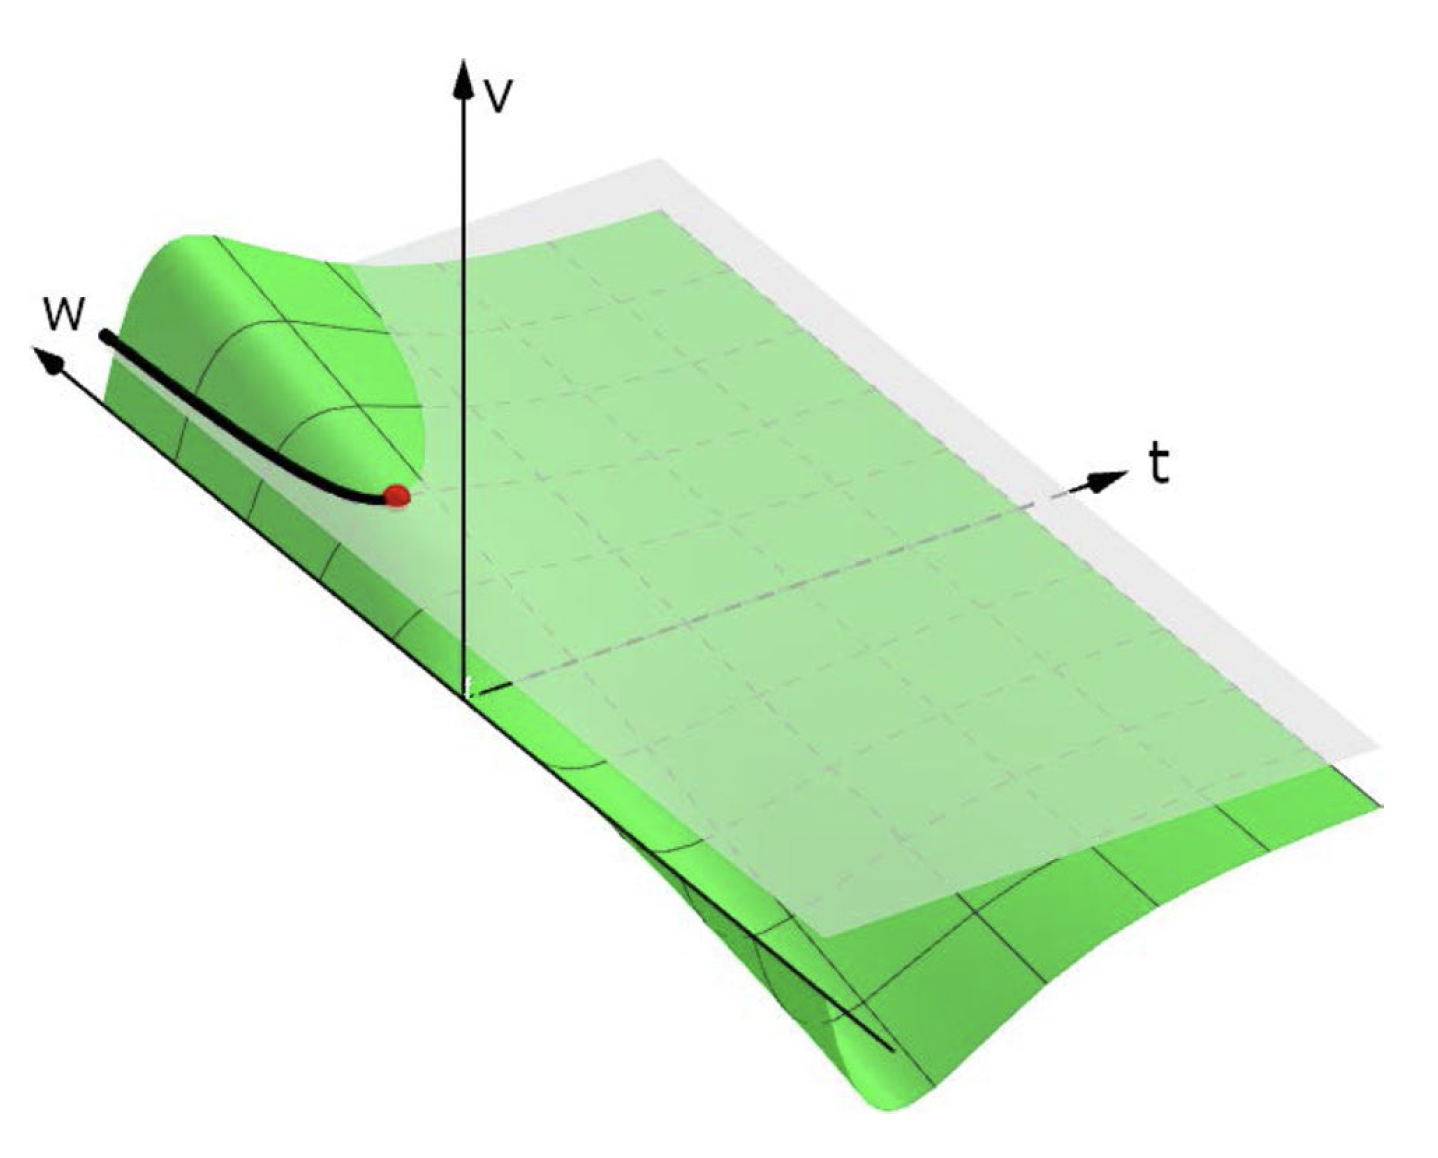
\includegraphics[width=0.6\textwidth]{figure5.png}
    \caption{\blue{In this sketch, the relation $V(t,W) - \vartheta =
        0$ defines an implicit function (black line along which $dV =
        0$). The critical point where the gradient diverges is shown
        in red}\label{fig1}}
    \end{figure}
  
  \blue{
\subsection{
  Membrane potential transition}
By considering the relations between
  $V^+$ , $V^-$ and $\dot{V}^+$, $\dot{V}^-$, we can derive the
  relation between $\frac{\partial V^+}{\partial
    w_{ji}}$ and $\frac{\partial V^-}{\partial w_{ji}}$ at each spike.
  Each spike at $t^{\text{post}}$ is triggered by a neuron's membrane potential
  crossing the threshold. We therefore have, at $t^{\text{post}}$,
  \begin{align}
    (V^-)_n - \vartheta = 0. \tag{35}
  \end{align}
  This relation defines $t^{\text{post}}$ as a differentiable function of $w_{ji}$ via the implicit function theorem (illustrated in
Fig. 5, see also [65]),  under the condition that $(\dot{V}^−)_n \neq
0$. Differentiation of this relation yields
\begin{align}
  \left(\frac{V^-}{d_{w_{ji}}}\right)_n + \left(\dot{V}^-\right)_n
\frac{d t^{\text{post}}}{d w_{ji}} = 0. \tag{36}
\end{align}
  }

The figure makes it quite intuitive that \blue{(35)} defines a
function $t^{\text{post}} (w)$ where \blue{(35)} is true. The implicit
function theorem gives the conditions on smoothness etc for which this
implicitly defined function is differentiable. Generally, \blue{(35)}
might not be expicitly solvable for $t^{\text{post}} (w)$ but one can
always take the derivative of  \blue{(35)} to find
\begin{align}
  \frac{\partial}{\partial w_{ji}} \left[(V^-(t^{\text{post}},W))_n -
    \vartheta\right] \\
 = \left(\frac{\partial V^-}{\partial w_{ji}}\right)_n + \left(\frac{\partial
    V^-}{\partial t^{\text{post}}}\right)_n \frac{d t^{\text{post}}}{d
    w_{ji}} = 0
\end{align}
which leads to \blue{(36)} as $\frac{\partial V^-}{\partial t^{\text{post}}} = \dot{V}^-$.

\blue{
  Since we only allow transitions for $(\dot{V}^−)_n \neq 0$, we have
  \begin{align}
    \frac{dt^{\text{post}}}{d w_{ji}} = -
      \frac{1}{\big(\dot{V}^-\big)_n} \left(\frac{\partial
        V^-}{\partial w_{ji}} \right)_n . \tag{37}
  \end{align}
  Note that corresponding relations were previously used to derive
  gradient-based learning rules for spiking neuron models [20–
    22,26,66]; in contrast to the suggestion in [20], Eq. (37) is not
  an approximation but rather an exact relation at all non-critical
  parameters and invalid at all critical parameters.  Because the
  spiking neuron’s membrane potential is reset to zero, we have
  \begin{align}
    \left(V^{+}\right)_n = 0. \tag{38}
  \end{align}
  This implies by differentiation
  \begin{align}
    \left(\frac{\partial V^+}{\partial w_{ji}}\right)_n +
    \big(\dot{V}^+\big)_n \frac{d t^{\text{post}}}{d w_{ji}} =
    0. \tag{39}
  \end{align}
}

I find the steps for $V^+$ slightly less intuitive but I think the
way to think about it is that while $t^{\text{post}}$ is defined
via the threshold condition on $V_-$, $V^+$ still is tied to
$t^{\text{post}}$ and hence depends on $t^{\text{post}}$. Maybe it
is actually easier to think about this backwards in time. If
integrated backwards, $V^+$ must reach $0$ at
$t^{\text{post}}$. That implies \blue{(39)} with all minus signs
... giving the same equation.

\blue{Using Eq. (37), this allows us to relate the partial derivative after the spike to the partial derivative before
  the spike,
  \begin{align}
    \left(\frac{\partial V^+}{\partial w_{ji}}\right)_n =
    \frac{\big(\dot{V}^+\big)_n}{\big(\dot{V}^-\big)_n}
    \left(\frac{\partial V^-}{\partial w_{ji}}\right)_n . \tag{40}
  \end{align}
}

This derives directly from substituting \blue{(39)} into \blue{(37)}.

\blue{
  Since we have $(V^+)_m = (V^-)_m$ for all other, non-spiking
  neurons $m \neq n$, it holds that
  \begin{align}
    \left(\frac{\partial V^+}{\partial w_{ji}}\right)_m + \big(
    \dot{V}^+\big)_m \frac{d t^{\text{post}}}{d w_{ji}} =
    \left(\frac{\partial V^+}{\partial w_{ji}}\right)_m + \big(
    \dot{V}^-\big)_m \frac{d t^{\text{post}}}{d w_{ji}} \tag{41}
  \end{align}
}

I suppose this just means that you can of course also ask what is the
derivative with respect to $w_{ji}$ of all the other $(V)_m$ at
$t^{\text{post}}$ ... just by asking this question at
$t^{\text{post}}$ makes $(V)_m$ a function of $t^{\text{post}}$.
    
\blue{
  Because the spiking neuron $n$ causes the synaptic current of all neurons $m \neq n$ to jump by $w_{mn}$ , we have
  \begin{align}
    \tau_{\text{mem}} \big(\dot{V}^+\big)_m = \tau_{\text{mem}}
    \big(\dot{V}^-\big)_m +w_{mn} \tag{42}
  \end{align}
  and therefore get with Eq. (36)
  \begin{align}
    \left(\frac{\partial V^+}{\partial w_{ji}}\right)_m =
    \left(\frac{\partial V^-}{\partial w_{ji}}\right)_m -
    \tau_{\text{mem}}^{-1} w_{mn} \frac{d t^{\text{post}}}{dw_ij}
    \tag{43} 
  \end{align}
  }

This equality results from reformatting \blue{(42)} into
\begin{align}
  \big(\dot{V}^-\big)_m - \big(\dot{V}^+\big)_m =
  - \tau_{\text{mem}}^{-1} w_{mn}
\end{align}
and inserting into \blue{(41)} reformatted as
\begin{align}
  \left(\frac{\partial V^+}{\partial w_{ji}}\right)_m =
  \left(\frac{\partial V^+}{\partial w_{ji}}\right)_m +  \Big(\big(
    \dot{V}^-\big)_m - \big(\dot{V}^+\big)_m \Big) \frac{d
      t^{\text{post}}}{d w_{ji}}
\end{align}

\blue{
  \begin{align}
    = \left(\frac{\partial V^-}{\partial w_{ji}}\right)_m +
  \frac{1}{\tau_{\text{mem}} (\dot{V}^-)_n} w_{nm}
  \left(\frac{\partial V^-}{\partial w_{ji}} \right)_n \tag{44}
  \end{align}
}
This is based on \blue{(37)} inserted into \blue{(43)} ... not
\blue{(36)}.

\blue{
  \subsection{Synaptic current transition}
  The spiking neuron $n$ causes the synaptic current of all neurons $m
  \neq n$ to jump by the corresponding weight $w_{mn}$ . We therefore have
  \begin{align}
    (I^+)_m = (I^-)_m + w_{mn} . \tag{45}
  \end{align}
  By differentiation, this relation implies the consistency equations
  for the partial derivatives $\frac{\partial I}{\partial w_{ji}}$
  with respect to the considered weight wji,
}

Essentially, $I^{\pm}$ is also a function of $t^{\text{post}}$ in the
same way as the other variables as they are tagged to the spike
time. So taking the same kind of derivative makes sense.

\blue{
  \begin{align}
    \left(\frac{\partial I^+}{\partial w_{ji}}\right)_m +
    \big(\dot{I}^+\big)_m \frac{d t^{\text{post}}}{d w_{ji}} =
    \left(\frac{\partial I^-}{\partial w_{ji}}\right)_m  +
    \big(\dot{I}^-\big)_m \frac{d t^{\text{post}}}{d w_{ji}} +
    \delta_{in}\delta_{jm}, \tag{46}
  \end{align}
  where $\delta_{ji}$ is the Kronecker delta.
}

Here the $\delta$'s arise because if $i=n$ and $j=m$, then
$\frac{\partial w_{mn}}{\partial w_{ji}} = 1 $ and it's $0$ in all
other cases.

\blue{
  Because
  \begin{align}
    \tau_{\text{syn}} \big(\dot{I}^+\big)_m =
    \tau_{syn}\big(\dot{I}^-\big)_m - w_{mn}, \tag{47}
  \end{align}
}

This comes from combining \blue{(45)} and the original current
dynamics \blue{(25b)}:
\begin{align}
  \tau_{\text{syn}} \dot{I}^+ - \tau_{\text{syn}} \dot{I}^- = -(I^+ -
  I^-)
\end{align}
by \blue{(25b)} and
\begin{align} 
(I^+)_m -  (I^-)_m = w_{mn}
\end{align}
by \blue{(45)}.

\blue{
  we get with Eq. (36)
  \begin{align}
    \left(\frac{\partial I^+}{\partial{w_{ji}}}\right)_m =
    \left(\frac{\partial I^-}{\partial w_{ji}}\right)_m +
    \tau_{\text{syn}^{-1}} w_{mn} \frac{d t^{\text{post}}}{d w_{ji}} +
    \delta_{in}\delta_{jm}, \tag{48} 
  \end{align}
}
This is based on \blue{(46)} and \blue{(47)}, where in \blue{(46)} one
shifts the $\big(\dot{I}^+\big)_m\frac{d t^{\text{post}}}{d w_{ji}}$
term to the right and then replaces $\big(\dot{I}^-\big)_m -
\big(\dot{I}^+\big)_m$ with $\tau_{\text{syn}^{-1}} w_{mn}$ based on \blue{(47)}.

\blue{
\begin{align}
  = \left(\frac{\partial I^i}{\partial w_{ji}}\right)_m -
  \frac{1}{\tau_{syn} \big(\dot{V}^-\big)_n} w_{mn}
  \left(\frac{\partial V^-}{\partial w_{ji}}\right)_n +
    \delta_{in}\delta_{jm}, \tag{49} 
\end{align}
}

This comes about by using \blue{(36)} to replace $\frac{d
  t^{\text{post}}}{d w_{ji}}$.

\blue{
  With $(I^+)_n = (I^-)_n$ and $\big(\dot{I}^+\big)_n =
  \big(\dot{I}^-\big)_n$, we have
  \begin{align}
    \left(\frac{\partial I^+}{\partial w_{ji}}\right)_n =
    \left(\frac{\partial I^-}{\partial w_{ji}}\right)_n. \tag{50}
  \end{align}
}
For the spiking neuron $n$, there are no self-synapses and hence the
synaptic current for this neuron does not change, and neither its
derivative. The equation \blue{(50)} then comes about by considering
the derivative of $(I^+)_n = (I^-)_n$,
\begin{align}
    \left(\frac{\partial I^+}{\partial w_{ji}}\right)_n +
    \big(\dot{I}^+\big)_n \frac{d t^{\text{post}}}{d w_{ji}} =
    \left(\frac{\partial I^-}{\partial w_{ji}}\right)_n  +
    \big(\dot{I}^-\big)_n \frac{d t^{\text{post}}}{d w_{ji}},
\end{align}
which together with $\big(\dot{I}^+\big)_n =
  \big(\dot{I}^-\big)_n$ gives the result.

    \subsection{Putting it all together}
  \blue{
    Using the relations of the partial derivatives from Eqs. (37), (40), (44), (49) and (50) in the transition equation
Eq. (34), we now derive relations between the adjoint variables. Collecting terms in the partial derivatives and
writing the index of the spiking neuron for the $k$th spike as $n(k)$, we
have
\begin{align}
  \xi_k = &\Bigg[ \sum_{m \neq n(k)} \left[ \tau_{\text{mem}}
      (\lambda^-_V - \lambda^+_V)_m \left(\frac{\partial V^-}{\partial
        w_{ji}}\right)_m
      +\tau_{\text{syn}} (\lambda^-_I - \lambda^+_I )_m
      \left(\frac{\partial I^-}{\partial w_{ji}}\right)_m
      - \tau_{\text{syn}} \delta_{in(k)} \delta_{jm} (\lambda^+_I)_m
      \right] \nonumber \\
    &+\left(\frac{\partial V^-}{\partial w_{ji}}\right)_{n(k)} \left[
      \tau_{\text{mem}} \left( \lambda^-_V -
      \frac{\big(\dot{V}^+\big)_{n(k)}}{\big(\dot{V}^-\big)_{n(k)}}
      \lambda_V^+ \right)_{n(k)}
      +\frac{1}{(\dot{V}^-)_{n(k)}} \left(\sum_{m \neq n(k)} w_{mn(k)}
      (\lambda_I^+- \lambda_V^+)_m - \frac{\partial l_p}{\partial
        t_k^{\text{post}}} + l_V^+ - l_V^- \right)\right] \nonumber \\
    &+ \tau_{\text{syn}} (\lambda^-_I - \lambda^+_I)_{n(k)}
    \left(\frac{\partial I^-}{\partial w_{ji}}\right)_{n(k)} \Bigg]
  \Bigg|_{t_k^{\text{post}}} . \tag{51}
\end{align} 
  }

This is a grand collection and reorganisation of terms from
\blue{(34)} and equations as listed. It is important to keep in mind
that in \blue{(34)} there are still scalar products of vectors
$\lambda_V^- \cdot \frac{\partial V^-}{\partial w_{ji}}$ and so on,
that in \blue{(51)} are broken up into their components and separately
into the $n(k)$ component of the spiking neuron and the $m \neq n(k)$
components of the non-spiking neurons. This is because the spiking and
non-spiking components have different relationships between
$\left(\frac{\partial V^+}{\partial w_{ji}}\right)_x$ and the ``minus
version'' $\left(\frac{\partial V^-}{\partial w_{ji}}\right)_x$. Note
that there is a typo in the manuscript that I have corrected above:
It's $w_{mn(k)}$, not $w_{n(k)m}$.

\blue{
  This form dictates the jumps of the adjoint variables for the
  spiking neuron n and all other, silent neurons $m$,
  \begin{align}
    (\lambda^-_V)_n &= \frac{\big( \dot{V}^+
      \big)_n}{\big(\dot{V}^-\big)_n} (\lambda_V^+)_n +
      \frac{1}{\tau_{\text{mem}} \big(\dot{V}^-\big)_n} \left[
        \sum_{m \neq n} w_{mn} (\lambda^+_V - \lambda^+_I)_m +
        \frac{\partial l_P}{\partial t_k^{\text{post}}} + l^-_V -
        l^+_V \right] , \tag{52a} \\
      (\lambda^-_V)_m &= (\lambda^+_V)_m \tag{52b} \\
      \lambda_I^- &= \lambda_I^+ \tag{52c}
  \end{align}
  With these jumps, the gradient reduces to
  \begin{align}
    \frac{d \cal L}{d w_{ji}} &= -\tau_{\text{syn}}
    \sum_{k=1}^{N_{\text{post}}} \delta_{in(k)} (\lambda_I)_j \tag{53}
    \\
    &= -\tau_{\text{syn}} \sum_{t \in \text{spikes from i}}
      (\lambda_I)_j(t) . \tag{54}
  \end{align}
}
These choices are now made to remove all the cumbersome terms from
\blue{(51)}. I have checked and the math works out that everything
is removed except the term with the $\delta$'s.

\blue{
  \subsection{Summary}
  The free adjoint dynamics between spikes are given by Eq. (32) while
  spikes cause jumps given by Eq. (52). The gradient for a given
  weight samples the post-synaptic neuron's  $\lambda_I$ when spikes are
  transmitted across the corresponding synapse [Eq. (53)]. Since we
  can identify, with $\big(\dot{V}^+\big)_n - \big(\dot{V}^-\big)_n =
  \tau_{\text{mem}}^{-1} \vartheta$,
  \begin{align}
    \frac{\big(\dot{V}^+\big)_n}{\big(\dot{V}^-\big)_n} =
    \frac{\big(\dot{V}^+\big)_n -
      \big(\dot{V}^-\big)_n}{\big(\dot{V}^-\big)_n} + 1 =
    \frac{\vartheta}{\tau_{\text{mem}} \big(\dot{V}^-\big)_n} + 1
    \tag{55}
  \end{align}
  the derived solution is equivalent to Eq. (2) and Table 2.

  \subsection{Fixed Input Spikes}
  If a given neuron $j$ is subjected to a fixed pre-synaptic spike train across a synapse with
weight $w_{j,\text{input}}$, the transition times are fixed and the adjoint
variables do not experience jumps. The gradient 
simply samples the neuron’s $\lambda_I$ at the times of spike arrival,
\begin{align}
  \frac{d \cal L}{d w_{j,\text{input}}} = - \tau_{\text{syn}}
  \sum_{t \in \text{input spikes}} (\lambda_I^+)_j(t) . \tag{56}
\end{align}
}
This is confusing and I am not sure entirely right. Jumps in $\lambda$
variables are caused by the integration boundaries of the piece-wise
integral in the loss function, broken at spike times. The jumps come
about if those spike times depend on the weight wrt which we are
taking a partial derivative. In this case, the spikes of the receiving
neuron $j$ depend on $w_{j,\text{input}}$ and hence should experience
jumps as normal when they spike. And their contribution to the
gradient is as described. The input spikes themselves do not cause
jumps -- but they also don't really have a neuron model attached or
any $\lambda$ adjoint variables. 
\blue{
\subsection{Coincident spikes}
The derivation above assumes that only a single neuron of the
recurrent network spikes at a given $t_k^{\text{post}}$. In general,
coincident spikes may occur. If neurons a and b spike at the same time
and the times of their respective threshold crossing vary
independently as function of $w_{ji}$ , the derivation above still
holds, with both neuron’s  $\lambda_V$ experiencing a jump as in
Eq. (52a).
}

I am not quite sure what it means for the two neurons' threshold
crossings to vary independently as a function of $w_{ji}$. But
presumably, even if this isn't always strictly true, it's probably so
rare and inconsequential that we don't need to worry about it in
practice.

\blue{
\section{Code availability}
Code to reproduce the shown results will be made available at https://github.com/eventprop.
}

\section{Summary}
The method is hence given as in tables 1 and 2: \\[0.2cm]
\noindent
Table 1: \\[0.2cm]
\noindent
\begin{tabular}{lll}
  \hline
  {\bf Free dynamics} & {\bf Transition condition} & {\bf Jumps at
    transition} \\
  \hline
$\tau_{\text{mem}} \frac{d}{dt} V = -V + I$ & $(V)_n - \vartheta = 0$,
  $\big(\dot{V}\big)_n \neq 0$ &
  $(V^+)_n = 0$ \\
  $\tau_{\text{syn}} \frac{d}{dt} I= -I$ & for any $n$ & $I^+= I^- + W
  e_n$ \\
  \hline
  \end{tabular}\\[0.5cm]
\noindent
Table 2: \\[0.2cm]
\noindent
\begin{tabular}{lll}
  \hline
  {\bf Free dynamics} & {\bf Transition cond.} & {\bf Jumps at
    transition} \\
  \hline
  $\tau_{\text{mem}} \lambda_V' = - \lambda_V - \frac{\partial
    l_V}{\partial V}$ & $t-t_k^{\text{post}} = 0$ &
  $(\lambda_V^-)_{n(k)} = (\lambda_V^+)_{n(k)} +
  \frac{1}{\tau_{\text{mem}} (\dot{V}^-)_{n(k)}} \Big[
      \vartheta (\lambda_V^+)_{n(k)}$ \\
      $\tau_{\text{syn}} \lambda_I' = -\lambda_I + \lambda_V$ & for
      any $k$ & $\hphantom{(\lambda_V^-)_{n(k)} = } + \left(W^T
      (\lambda_V^+ - \lambda_I^+)\right)_{n(k)} + \frac{\partial
        l_p}{\partial t_k^{\text{post}}} + l_V^- - l_V^+ \Big]$ \\
  \hline
\end{tabular} \\[0.5cm]
The gradient is then calculated as
\begin{align}
  \frac{d \cal L}{d w_{ji}} = - \tau_{\text{syn}} \sum_{t \in
    \text{spikes of neuron }
    i} (\lambda_I^+)_j (t) 
\end{align}
Similar for input spikes (see \blue{(56})).

\newcommand{\liexp}{\exp\left(-t^{\text{post}}_{i,l(i)}/\tau_0\right)}
\newcommand{\liexpb}{\exp\left(t^{\text{post}}_{i,l(i)}/\tau_1\right)}
\newcommand{\smexp}{\sum_{k=1}^3 \exp\left(-t^{\text{post}}_{i,k}/\tau_0\right)}
\subsection{Ying-Yang experiment}
For the Ying-Yang experiment, Pehle et al. use the loss function:
\begin{align}
  {\cal L}= - \frac{1}{N_{\text{batch}}}
  \left[\sum_{i=1}^{N_{\text{batch}}} \log \left[
      \frac{\liexp}{\smexp}\right] - \alpha
    \left[\liexpb -1 \right] \right]
\end{align} 
This is a loss function that is of the form $\sum l_p(t_k)$. For the
backwards jumps, we need
\begin{align}
  \frac{\partial \cal L}{\partial t_{i,l(i)}} &= -
  \frac{1}{N_{\text{batch}}} \left[\frac{\smexp}{\liexp}
    \left(\frac{-\frac{1}{\tau_0} \liexp}{\smexp} \right. \right.\\
   & \hphantom{= -\frac{1}{N_{\text{batch}}}} \left. \left.
    -\frac{\liexp}{\left(\smexp\right)^2}
    \left(-\frac{1}{\tau_0}\liexp\right)\right) - \alpha
    \frac{1}{\tau_1} \liexpb \right] \\
  &= -
  \frac{1}{N_{\text{batch}}} \left[ -\frac{1}{\tau_0} +
    \frac{1}{\tau_0}\frac{\liexp}{\smexp} -\frac{\alpha}{\tau_1}\liexpb
    \right] \\
  &= 
  \frac{1}{N_{\text{batch}}} \left[\frac{1}{\tau_0} \left(1 -
    \frac{\liexp}{\smexp} \right) + \frac{\alpha}{\tau_1}\liexpb
    \right] \label{eq:lyy1} \\
  \frac{\partial \cal L}{\partial t_{i,j}} &= -
  \frac{1}{N_{\text{batch}}} \left[\frac{\smexp}{\liexp} \left(-\frac{\liexp}{\left(\smexp\right)^2}\right)
    \left(-\frac{1}{\tau_0}\exp\left(-t^{\text{post}}_{i,j}/\tau_0\right)
    \right)\right] \\
  &=  
  \frac{1}{N_{\text{batch}}} \left[ - \frac{1}{\tau_0}
    \frac{\exp\left(-t^{\text{post}}_{i,j}/\tau_0\right)}{\smexp} \right]\label{eq:lyy2} 
\end{align}
We will use (\ref{eq:lyy1}) and (\ref{eq:lyy2}) to update $\lambda_V$
at jump points of output neurons.

\section{MNIST example}
Here the authors define the cost function
\begin{align}
  {\cal L} = - \frac{1}{N_{\text{batch}}} \sum_{i=1}^{N_{\text{batch}}} \log \left[ \frac{\exp\left(\max_t V_{l(i)} (t)\right)}{\sum_{k=1}^{10} \exp\left(\max_t V_k(t)\right)} \right]
\end{align}
where $V_k(t)$ is the voltage trace of the $k$th readout neuron, $l(i)$ is the index of the correct label for the $i$th sample and $N_{\text{batch}}$ is the number of samples ina  given batch.

They then argue: \blue{`` Note that we can write the maximum voltage as $\max_t V_k(t) = \int V_k(t) \delta(t-t_{\text{max}} dt$ with the time of the maximum $t_{\text{max}}$ and the Dirac delta $\delta$, allowing us to apply the chain rule to find the jump of $\lambda_{V_k}$ (cf Table 2) at time $t_{\text{max}}$ (terms containing the distributional derivative of $\delta$ are always zero).''}

The first observation is that this does not conform to their general expression for {\cal L},
\begin{align}
  {\cal L} = l_p(t^{\text{post}}) + \int_0^T l_V(V(t),t) dt
\end{align}
so the normal formula do not apply. However, I believe the argument is that if one did the derivation for this different form of cost function, using the represnetation of $\max_t V_k(t)$ with the Dirac delta as explained above, one would arrive at a similar set of update equations where there si a jump in $\lambda_{V_k}$ at $t_{max,k}$ 

This seems supported by the helpful comment in the earlier discussion: \blue{The loss $l_V$ may depend on the voltage at a discrete time $t_i$ using the Dirac delta,
$l_V (V(t), t) = V(t) \delta(t_i − t)$ , causing a jump of $\lambda_V$ of magnitude $\tau_{\text{mem}}^{-1}$ at time $t_i$. Note that in many practical
scenarios as found in deep learning, the loss $l_V$ depends only on the state of a constant number of neurons, irrespective of network size. If $l_V$ depends on the voltage of non-firing readout neurons, we have $ l^+_V = l^−_V$ and the corresponding term in the jump given in Table 2 vanishes.}

In order to unpick the details of what's needed, let us define $M_k = \max_t V_k (t)$ such that
\begin{align}
  {\cal L} &= - \frac{1}{N_{\text{batch}}} \sum_{i=1}^{N_{\text{batch}}} \log \left[ \frac{\exp\left(M_{l(i)}\right)}{\sum_{k=1}^{10} \exp\left(M_{k}\right)} \right] \\
  &= - \frac{1}{N_{\text{batch}}} \sum_{i=1}^{N_{\text{batch}}} M_{l(i)} - \log\left(\sum_{k=1}^{10} \exp\left(M_{k}\right)\right) 
\end{align}
and the partial derivatives with respect to $V_r$ and $V_{l(i)}$ would be obtained by the chain rule, for $V_r(t)$ in presentation $i$ and $r \neq l(i)$,
\begin{align}
  \frac{\partial}{\partial V_r(t)} {\cal L} &= -\frac{1}{N_{\text{batch}}}  \left(-\frac{\exp\left(M_r\right)}{\sum_{k=1}^{10} \exp\left(M_{k}\right)}\right)\frac{\partial}{\partial V_r} M_r
\end{align}
where
\begin{align}
  \frac{\partial}{\partial V_r(t)} M_r &= \frac{\partial}{\partial V_r(t)}  \int V_r(t') \delta(t'-t_{\text{max}}) dt' \\
  &=  \int \delta(t'-t)\delta(t'-t_{\text{max}}) dt' \\
  &= \delta(t-t_{\text{max}})
\end{align}
which, if inserted into the reverse differential equation for $\lambda_V$ in Table 2, would lead to the described jump behaviour. In this case the jump would be
\begin{align}
 - \frac{1}{\tau_{\text{mem}}} \frac{1}{N_{\text{batch}}} \frac{\exp\left(M_r\right)}{\sum_{k=1}^{10} \exp\left(M_{k}\right)}
\end{align}
at time $t_{\text{max,r}}$ (the minus sign is from the $\lambda_V$ equation in Table 2: $-\frac{\partial l_V}{\partial V}$).

For the voltage of the correct output neuron, $V_{l(i)}$ the derivative would be
\begin{align}
  \frac{\partial}{\partial V_{l(i)}(t)} {\cal L} &= -\frac{1}{N_{\text{batch}}}  \left(1 - \frac{\exp\left(M_{l(i)}\right)}{\sum_{k=1}^{10} \exp\left(M_{k}\right)}\right)\frac{\partial}{\partial V_{l(i)}} M_{l(i)}
\end{align}
and hence the jump,
\begin{align}
\frac{1}{\tau_{\text{mem}}} \frac{1}{N_{\text{batch}}} \left(1 - \frac{\exp\left(M_{l(i)}\right)}{\sum_{k=1}^{10} \exp\left(M_{k}\right)}\right)
\end{align}
at time $t_{\text{max,r}}$ (including the minus sign from table 2, as above).

So, in essence, in the MNIST example with non-spiking output neurons, there are no spike times to jump at. Furthermore, $l_V$ does not jump at other neurons' spike times, so there is no contribution $l_V^- - l_V^+$ to other neurons' jumps. However, in addition to their normal exponential decay $\lambda_V$ equation, output neurons jump at their $t_{\text{max}}$ by the amounts noted above. $t_{\text{max}}$ can obviously easily be recorded in the forward pass.

The same technology can be applied to the spiking Heidelberg digits dataset. Though (as of 2022-02-15) not with much success.

\section{Derivation of exact solution for $\lambda_V$ and $\lambda_I$
  within a timestep}

\begin{align}
  \tau_m \lambda'_V = -\lambda_V \label{eqn:lv1} \\
  \tau_{\text{syn}} \lambda'_I = - \lambda_I + \lambda_V
\end{align}
From equation (\ref{eqn:lv1}) we easily get
\begin{align}
  \lambda_V(t+ \Delta t - t') = \lambda_V(t+\Delta t) \exp\left(-\frac{t'}{\tau_m}\right).
\end{align}
Then we have
\begin{align}
  \lambda'_I = \frac{1}{\tau_{\text{syn}}} \left(-\lambda_I +
  \lambda_V(t+\Delta t) \exp\left(-\frac{t'}{\tau_m}\right)\right)
\end{align}
The solution to the autonomous equation is
\begin{align}
  \lambda_I = \tilde{\lambda}_I \exp\left(-\frac{t'}{\tau_{\text{syn}}}\right)
\end{align}
and with the usual trick $\tilde{\lambda}_I \rightarrow
\tilde{\lambda}_I(t)$ we get
\begin{align}
  \lambda'_{I} &= \tilde{\lambda}'_I \exp\left(-\frac{t'}{\tau_{\text{syn}}}\right) - \frac{1}{\tau_{\text{syn}}} \tilde{\lambda}_I \exp\left(-\frac{t'}{\tau_{\text{syn}}}\right) = - \frac{1}{\tau_{\text{syn}}}
  \lambda_I + \tilde{\lambda}'_I \exp\left(-\frac{t'}{\tau_{\text{syn}}}\right)
\end{align}
Hence, we can identify
\begin{align}
  \tilde{\lambda}'_I \exp\left(-\frac{t'}{\tau_{\text{syn}}}\right) &= \frac{1}{\tau_{\text{syn}}}
  \lambda_V =
  \frac{1}{\tau_{\text{syn}}} \lambda_V(t+\Delta t) \exp\left(-\frac{t'}{\tau_m}\right) \\
 \Rightarrow \quad  \tilde{\lambda}'_I &= \frac{1}{\tau_{\text{syn}}}
  \lambda_V(t+\Delta t)
  \exp\left(-\left(\frac{1}{\tau_m}-\frac{1}{\tau_{\text{syn}}}\right)
  t' \right) \\
\Rightarrow \quad  \tilde{\lambda}_I &= - \frac{1}{\frac{1}{\tau_m} -
  \frac{1}{\tau_{\text{syn}}}} \frac{1}{\tau_{\text{syn}}} \lambda_V(t+\Delta t) \exp\left(-\left(\frac{1}{\tau_m}-\frac{1}{\tau_{\text{syn}}}\right)t' \right) +C \\
  \Rightarrow \quad  \lambda_I &= - \frac{\tau_m}{\tau_{\text{syn}}-\tau_m} \lambda_V(t+\Delta t) \exp\left(-\left(\frac{1}{\tau_m}-\frac{1}{\tau_{\text{syn}}}\right)
  t' - \frac{t'}{\tau_{\text{syn}}}\right) + C
  \exp\left(-\frac{t'}{\tau_{\text{syn}}}\right) \\
  &= - \frac{\tau_m}{\tau_{\text{syn}}-\tau_m} \lambda_V(t+\Delta t)
  \exp\left(-\frac{t'}{\tau_m}\right) + C
  \exp\left(-\frac{t'}{\tau_{\text{syn}}}\right) 
\end{align}
At $t' = 0$,
\begin{align}
  - \frac{\tau_m}{\tau_{\text{syn}}-\tau_m} \lambda_V(t+\Delta t) + C
  &= \lambda_I(t+\Delta t) \\
  \Rightarrow \quad  C &= \lambda_I(t+\Delta t)  +
  \frac{\tau_m}{\tau_{\text{syn}}-\tau_m} \lambda_V(t+\Delta t)
\end{align}
and hence
\begin{align}
  \lambda_I = \frac{\tau_m}{\tau_{\text{syn}}-\tau_m}
  \lambda_V(t+\Delta t)  \left(\exp\left(-\frac{t'}{\tau_{\text{syn}}}\right) - \exp\left(-\frac{t'}{\tau_m}\right)\right) + \lambda_I(t+\Delta t) \exp\left(-\frac{t'}{\tau_{\text{syn}}}\right)
\end{align}
And accordingly for $t' = \Delta t$,
\begin{align}
  \lambda_V (t) &= \lambda_V(t+\Delta t) \exp\left(-\frac{\Delta
    t}{\tau_m}\right) \\
  \lambda_I (t) &= \frac{\tau_m}{\tau_{\text{syn}}-\tau_m}
  \lambda_V(t+\Delta t)  \left(\exp\left(-\frac{\Delta
    t}{\tau_{\text{syn}}}\right) - \exp\left(-\frac{\Delta
    t}{\tau_m}\right)\right) + \lambda_I(t+\Delta t)
  \exp\left(-\frac{\Delta t}{\tau_{\text{syn}}}\right)
\end{align}

 As the forward equations are identical for $V$ (i.e. like the $\lambda_I$ equation), the equivalent equation can be used for $V$ in the forward pass.

\section{GeNN Implementation Notes (Outdated?)}
\begin{itemize}
\item In the normal forward pass we need to save:
  \begin{itemize}
    \item spike times (could be the normal spike time recording bit array)
    \item $(-V+I)_{n(k)}(t_k^{\text{post}})$ i.e. the input current
      minus voltage (to represent $\tau_{\text{mem}}
      (\dot{V}^-)_{n(k)}$) at each spiking neuron when a spike is
      detected (before reset). This could be done as part of the reset
      code but we need a new data structure for it. A per neuron ring
      buffer to hold data for an estimated maximum number of spikes?
    \item We also need $l_V^- - l_V^+$ at times $t_k^{\text{post}}$,
      which I guess is relevant when the spiking neuron's $V$
      contributes to the voltage-dependent loss. At other spike times
      the relevant $V$'s should be continuous and the difference
      $0$. This data is one number for all neurons. One would probably
      save it for all spike times. In a egp ring buffer?
  \end{itemize}
\item I imagine a separate ``backward pass'', probably to be added as
  an additional feature to GeNN, in which
  \begin{itemize}
  \item The $\lambda$ continuos dynamics is integrated backward with Euler
    time steps as usual. This could be entered by users as a
    ``backward\_sim\_code''
  \item Spikes are retrieved from the spike recording buffer into
    the current spikes buffer (in an inversion of the usual
    recording code)
  \item There would be a ``backward\_reset\_code'' where all
    spiking neurons get the jumps applied. This will access the
    $-V+I$ buffer and step back the counter on it.
  \item All synapses execute their ``backward\_sim\_code'' which
    adds the $-\tau_{\text{syn}} \lambda_{I,\text{post}}$ value to
    their ``gradient'' variable that respresents $\frac{d \cal
      L}{d w_{ji}}$.
  \end{itemize}
\item At the end of the ``backward pass'', all synapse weights get updated
  with $-\eta \cdot \text{gradient}$.
\end{itemize}

  We could also try to hack it where, depending on a flag, either
  forward or backward things happen within normal sim\_code etc
  structures.  But a) what do we do about the additional data
  structures, especially the per-neuron one? and b) how would we
  handle the retrieving of spikes into the current spike array
  efficiently? Also, would we need to do something awkward about the
  time variable?

\section{Insight of the day 2022-02-16}
  Do {\em not} taper the learning rate aggressively (\verb+p["ETA_DECAY"]= 0.95+) while at the same time using an Adam optimizer. Should have known this. Removing the decay, with not too unusual settings otherwise, now reached almost 60\% training correct. Though now some over-fitting has become evident in lower evaluation set scores. This fits the narrative from teh eprop work.

  TODO: Re-investigate different regularisations ...

\end{document}
